\documentclass[British]{article}
\usepackage[dvipsnames]{xcolor}
\usepackage[utf8]{inputenc}
\usepackage[british]{babel}
\usepackage{siunitx,etoolbox}
\usepackage[export]{adjustbox}
\usepackage{dblfloatfix}
\usepackage{lmodern}
\usepackage{float}
\usepackage{url}
\usepackage{color}
\usepackage{listings}
\usepackage{graphicx}
\usepackage{graphics}
\usepackage{hyperref}
\usepackage{wrapfig}
\usepackage{fancyhdr}
\usepackage{natbib}
\lstset{
   language=Java,
   aboveskip=3mm,
   belowskip=3mm,
   showstringspaces=false,
   columns=flexible,
   basicstyle={\small\ttfamily},
   numbers=none,
   numberstyle=\tiny\color{cyan},
   keywordstyle=\color{blue},
   commentstyle=\color{green},
   stringstyle=\color{red},
   tabsize=1
   }

\fancyhf{}
\fancyfoot[c]{Page \thepage \hspace{1pt} of \pageref{LastPage}}
\pagestyle{fancy}
\setcitestyle{numbers}
%\title{
   % {Paths: A Branching Storyline Game} \\
    %{\large IDATG2001 Programmering 2 Exam}\\
    %{\begin{figure}[H]
     %\centering
      %\includegraphics[width=13cm,trim={0 0 0 {5\wd}}]{figures/Paths_main_menu.png}
       %\caption {Paths main menu. Source: Primary.}
        %\end{figure}} 
%}
%\author{Erik Bjørnsen & Emil Klevgård-Slåttsveen}
%\date{23.May.2023}
%\begin{document}

%\maketitle

%\tableofcontents
%\newpage 

\title{Paths: A Branching Storyline Game \\
\large IDATG2001 Programming 2 Exam}
\author{Erik Bjørnsen \& Emil Klevgård-Slåttsveen}
\date{23.May.2023}

\begin{document}
\maketitle

\begin{figure}[h]
  \centering
  \includegraphics[width=13cm, trim={0 0 0 5cm}]{figures/Paths_main_menu.png}
  \caption{Paths main menu. Source: Primary.}
\end{figure}

\newpage 
\tableofcontents

\newpage 


\begin{abstract}
    %The abstract should be an extremely condensed version of the report. Think one sentence with the main message from each of the chapters of the body matter as a starting point. landes1951scrutinyempty citation have given some very nice instructions on how to write a good abstract.
    Have you ever tried playing a narrative branching game with endings based on your own choices? Well, if you are interested, try the new Paths game that we have created for our final exam project for the IDATG2001 Programming 2 course at NTNU. If you read this report you will hear about the development process of this game, starting with an introduction to the game genre in the modern gaming industry. In the following chapters you will first read about some of the most common theories within the field that are central in the development process. Then there will be a description of our contribution with focus on the requirements, the technical design choices and also which tools and methods that were applied for the project management. Nearing the end of the report there are chapters that will give you a insight in the overall implementation of the program code and the testing and deployment of it. Finally there will be a discussion and conclusion, where we will evaluate and summarise the project and its results. 
\end{abstract}

\section{Introduction}
In the gaming industry, there have been several popular games that have been based on narrative branching. Narrative branching in games is in most cases tightly connected with the player's choices throughout the story, which greatly affects the game ending. Some great examples are Rockstar Games' Grand Theft Auto 5 (2013), Rockstar Games' Red Dead Redemption 2 (2018) and Square Enix's External Studios' Life is Strange (2015)\cite{miller2023}. A common factor for these games, is that they all include a narrative branching mechanism, that contains consequences for the players actions. These consequences often appear in dialog decisions while interacting with NPCs, when committing crimes or showing kindness to others, and they often greatly change the played character's personality. In addition these games also include some decisions connected to the difficulty of some missions according to the player's gear level, physical attributes and which teammates you choose. In this project we have chosen to simplify the structure of these games' narrative branching mechanisms to make a branching storyline game, with a much simpler GUI. Throughout the development process of this game we have taken many critical choices in relation to the game's structure, which design choices and principles we have chosen to develop this game, that we will review in this report.

\subsection{Definitions, Acronyms and Abbreviations}

\begin{center}
\makebox[1 \textwidth][c]{ 
\begin{tabular}{ |c|c| } 
\hline
\bfseries Definitions, Acronyms, or abbreviations & \bfseries Explanation \\
\hline 
NPC & Non-player character\\ 
\hline
GUI & Graphical user interface\\ 
\hline
OOP & Object-Oriented Programming \\
\hline
MVC & Model-view-controller \\
\hline
DAO & Data Access Object \\
\hline
VCS & Version Control System \\
\hline
IDE & Integrated Development Environment  \\
\hline
AAA & Arrange, Act and Assert \\
\hline
\end{tabular}
}
\end{center}


\section{Background}

\subsection{Encapsulation}
In object oriented programming there are some important principles that ensure the robustness of the software and the encapsulation of the information in the software's components. The most important principles in this category are coupling and cohesion. Coupling is a principle that strives to separate the different components in the project to create a loose coupling between them \cite[p.~266]{barnes2017objects}. There is also a subcategory of coupling called "implicit coupling", which primarily occurs when two classes are tightly coupled, the classes' information access types are dependant of each other, and are declared public. If you were to change one of these fields from public to private, the code would not compile anymore \cite[p.~274]{barnes2017objects}. 
\\\\
Cohesion on the other hand is essential to achieve independent and strong components in a program. Cohesion is achieved by making classes or methods responsible for one well defined task \cite[p.~278]{barnes2017objects}. An example of this might be a program that has a class that represents the player and a class that represents a player-register. The player class should then only have getter and setter methods for the players' attributes and no list for the different players, since that should be the player-register's responsibility. This is valuable to ensure more structured and understandable code lines, and it constitutes a great difference in the applications robustness in combination with the coupling. 

\newpage

\begin{wrapfigure}{r}{0.6\textwidth}
\begin{center}
      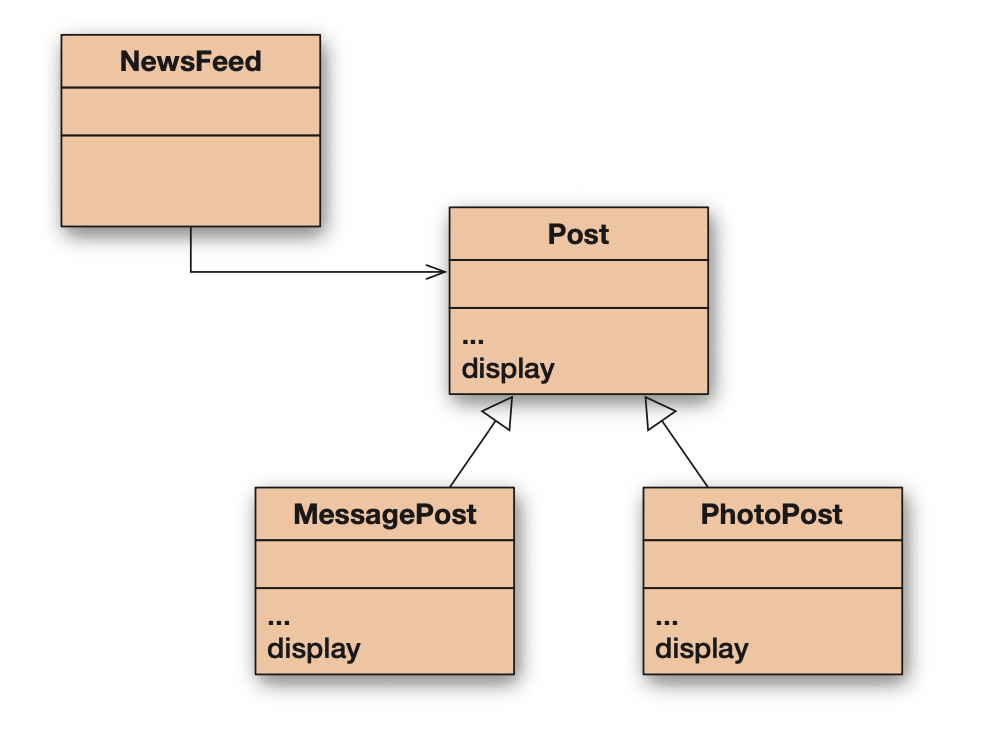
\includegraphics[width=0.47\textwidth]{figures/post_system.png} 
   \caption{
Messaging system inheritance hierarchy. Source: \cite[p.~368]{barnes2017objects}.
}
\end{center}
\end{wrapfigure}
%Må kanskje skrive Inheritance kapittelet pga. antall ord

%\subsection{Inheritance and Abstraction}
%To help find solutions with encapsulation problems in OOP, it can be very useful to separate responsibilities of the different classes by using inheritance to amplify the impact of coupling and cohesion. Inheritance makes it possible to implement a class as an extension of another to solve problems with code duplication \cite[p.~343]{barnes2017objects}. This is done by creating a superclass, which works as "the ancestor" in the inheritance hierarchy, that lets subclasses extend (inherit) the superclass' abilities (see examples to the right). Inheritance  gives great advantages in ensuring code reuse, easier maintenance and extendibility for future releases \cite[pp.~351-352]{barnes2017objects}. 
%\begin{wrapfigure}{l}{0.6\textwidth}
%\begin{center}
      %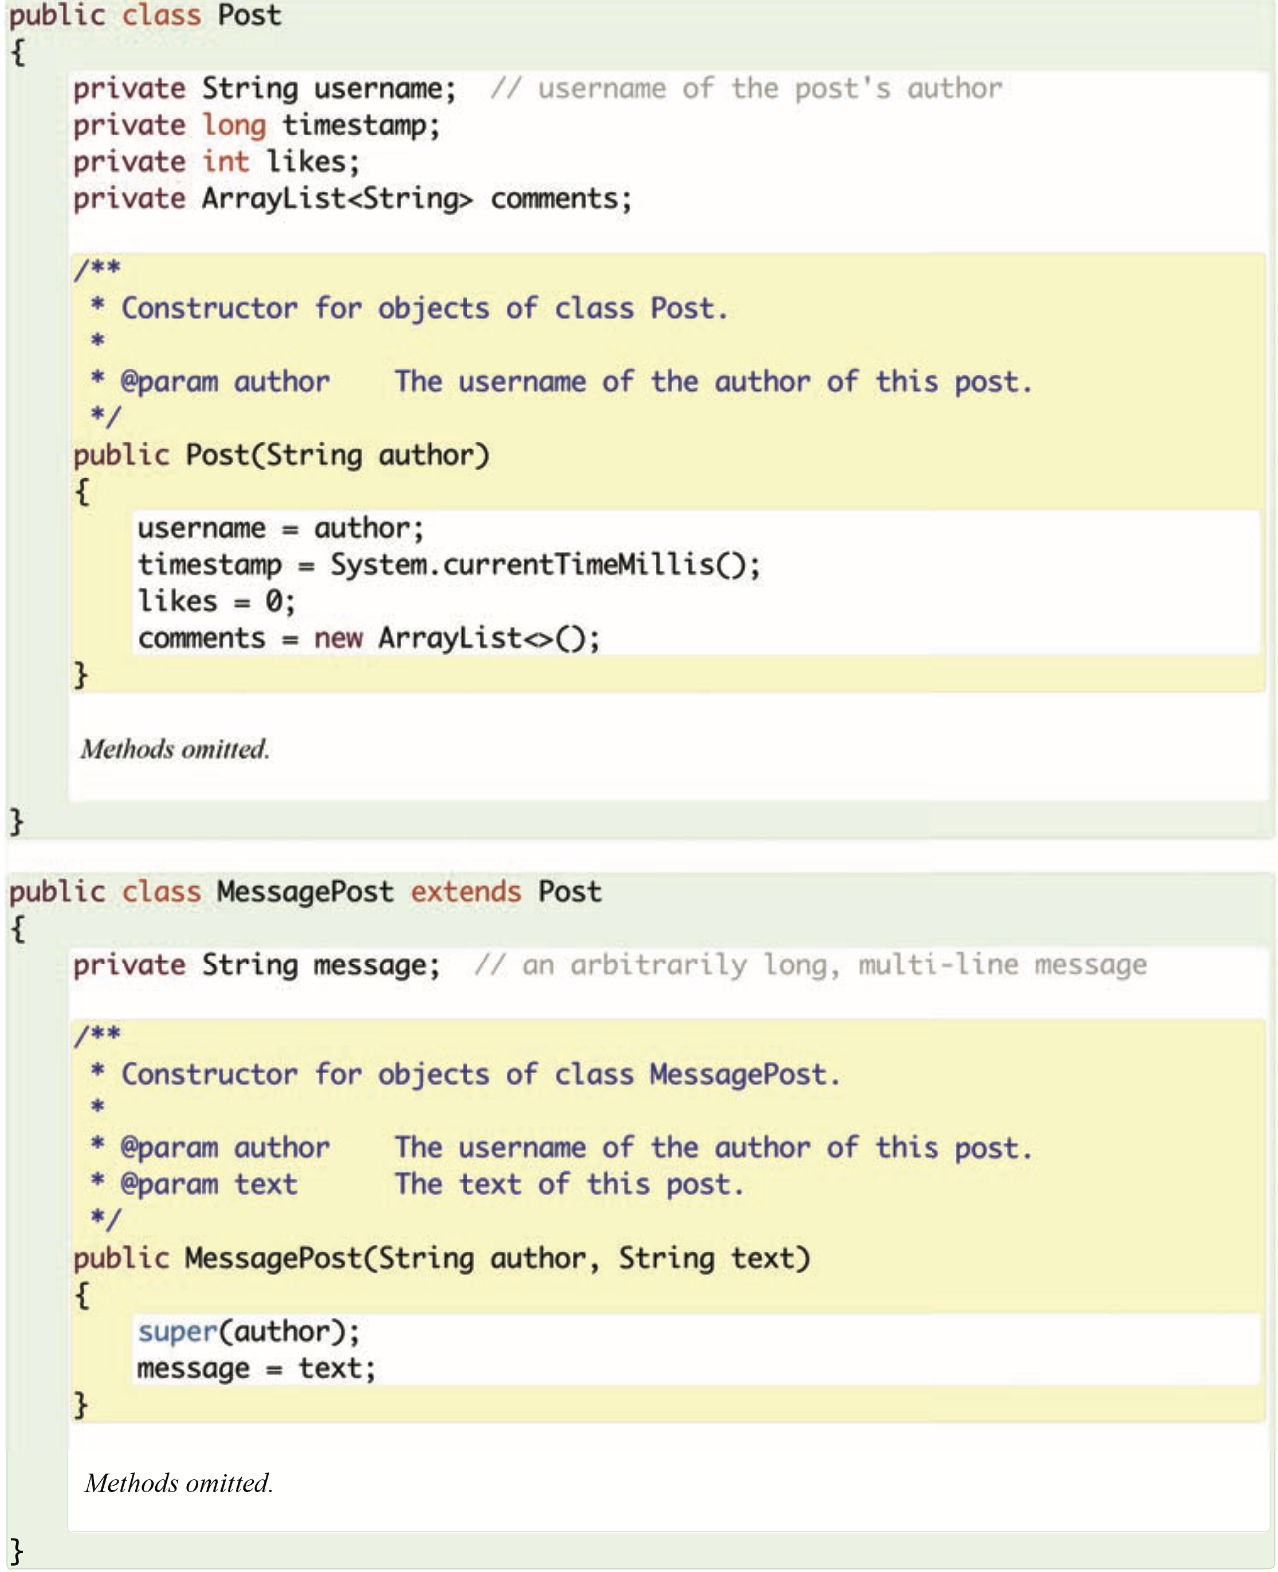
\includegraphics[width=0.47\textwidth]{figures/Post_class_image.png} 
  % \caption{
%Messaging system classes. Source: \cite[p.~348]{barnes2017objects}.
%}
  % \end{center}
%\end{wrapfigure}

%An example of this is a messaging system where there are one class for creating message-posts with only text and one class for creating photo-posts with only photos. Both of these classes will have very similar constructors, and to avoid code duplication these classes can inherit their common fields from a superclass called Post by calling the "super();" command in each of the subclass' constructors (see the image to the right). Inheritance also gives great advantages in ensuring code reuse, easier maintenance and extendibility for future releases \cite[pp.~351-352]{barnes2017objects}. 

\subsection{Abstraction}
In addition to Encapsulation there is also another theory central to OOP, called Abstraction. Abstraction makes it possible to reduce the complexity of the classes in a inheritance hierarchy down to their most essential contents. This can be done by using interfaces, that are characterised by making it possible to switch out the class keyword with the interface keyword. Interfaces do not contain any constructors or instance fields, all methods have public visibility regardless of their keyword and methods marked with a static or default method body. In addition interfaces make it possible for classes to implement more than one interface at the time, which makes it different from inheritance, that only lets classes inherit one superclass at a time \cite[pp.~417-418]{barnes2017objects}. Barnes and Kölling give an example of multiple inheritance that can be found on page 420: 
\begin{lstlisting}
public class Hunter implements Actor, Drawable
{

}
\end{lstlisting}
Here the class Hunter implements the interfaces Actor and Drawable, and it must therefore override both of the interfaces' methods. Implementing these interfaces lead to a more extendable structure with more flexibility, due to the cleanly separated type specification that creates less coupling when implemented \cite[p.~428]{barnes2017objects}. 

%Polymorphism må muligens fjernes pga. for mange ord

%\subsection{Polymorphism}
%Often when using inheritance we face problems related to how the hierarchy's object only can be inherited in one direction, from the superclass and down to the subclasses, and therefore the superclass does not know of the subclasses fields and their types. This is a typical case where polymorphic variables come in handy, but to understand it we need to know the difference between which objects in the hierarchy that are statically or dynamically typed. Polymorphism is a Greek word that means "many-shaped", which essentialy is what polymorphism helps us with, storing objects of many shapes or forms in variables\cite{microsoft2023}. The static type (static representation of the program) is typically the declared type of the variable in the source code, for example:
%\begin{lstlisting}
%ArrayList<String> stringList = new ArrayList<>();
%\end{lstlisting}
%Here the ArrayList type is the same both for the varible type of stringList, and for the object stored in the variable. If the type of the variable would be dynamically typed (dynamic behaviour of the program), the variable would be the type of the object it is assigned to at run-time, for example:
%\begin{lstlisting}
%Post post = new MessagePost();
%\end{lstlisting}

%\begin{wrapfigure}{r}{0.65\textwidth}
%\begin{center}
  %    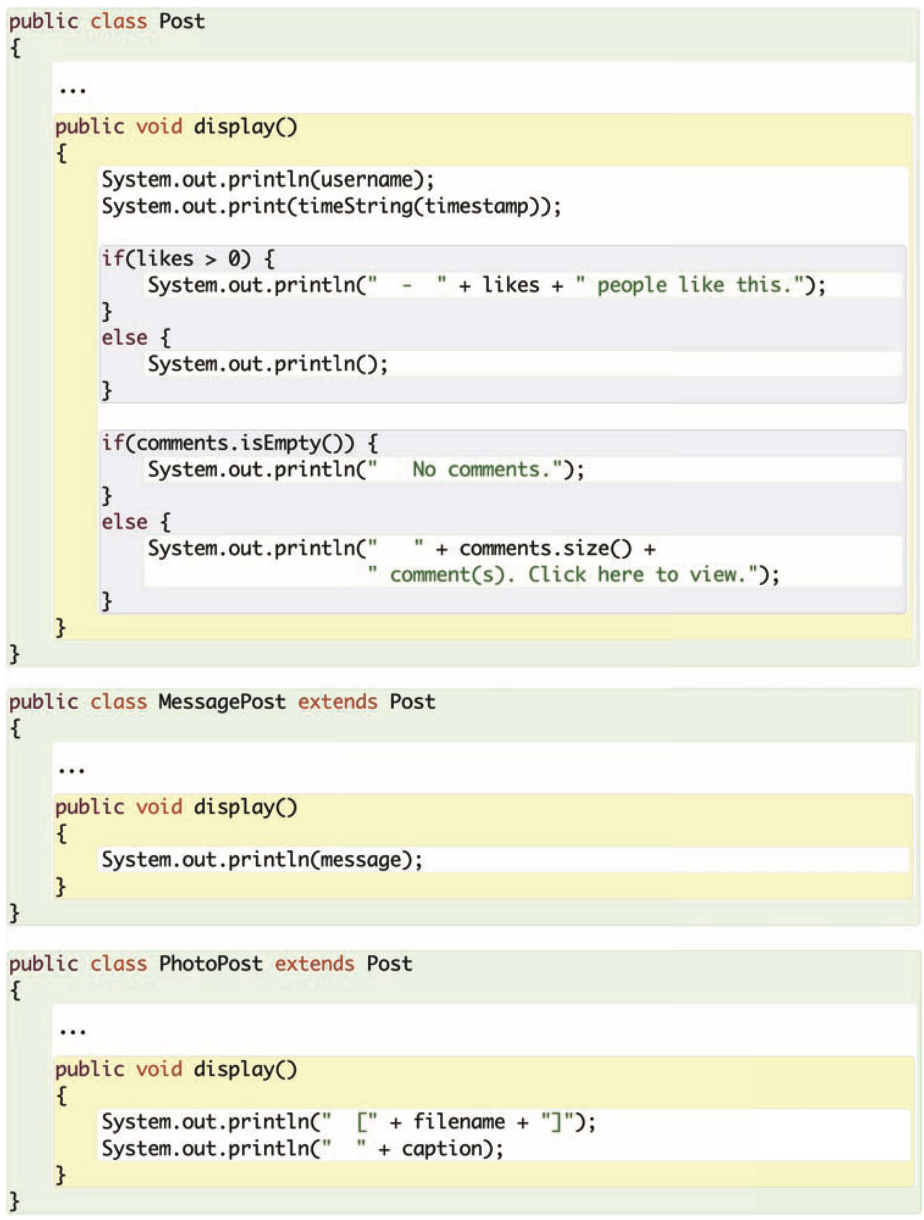
\includegraphics[width=0.47\textwidth]{figures/Display_method.png} 
 %   \caption{
%Display method overrides. Source: \cite[p.~369]{barnes2017objects}.
%}
   % \end{center}
%\end{wrapfigure}
%In this case the type of the variable post is Post, but the type of the object stored in post is MessagePost \cite[p.~365-367]{barnes2017objects}. Polymorphism is also central in  method overriding. Method overriding is when there is a method defined in a superclass which is written with the exactly same signature as the method defined in the superclass but with a "@Override" annotation to make it clear that it is a new version of the method in the superclass (See image to the right) \cite[p.~370]{barnes2017objects}. On page 385 Barnes and Kölling write that by achieving this we can ensure that all specialised methods are invoked for every particular subtype, so that objects from different classes can be clearly activated by the same method call. 

%Abstarction delen må muligens fjernes pga. for mange ord

%\subsection{Abstraction}
%The last of the four foundational pillars in OOP amplifies the concepts of inheritance and polymorphism and is known as abstraction. Abstraction makes it possible to create abstract classes and interfaces in order to reduce the complexity of the classes in a inheritance hierarchy down to their most essential contents. Abstract classes are characterised by being able to be prefixed by the "abstract" keyword, having no method bodies and not being able to be instantiated. These characteristics are very useful in combination with inheritance and polymorphism since we not always want to create objects of the superclass since it often becomes very general and concrete in many cases. An example of this is a animal hierarchy where the Animal superclass has a method called "act()" which the animal subclasses of Fox and Rabbit can override. The problem here is that you can also use the Animal class' act method which is very illogical, since the Animal class is not a specific animal itself with any common characteristics \cite[pp.~406-409]{barnes2017objects}. Interfaces on the other hand are characterised by making it possible to make switch out the class keyword with a interface keyword, they do not contain any constructors or instance fields, all methods have public visibility regardless of their keyword (whether concrete, static or abstract),methods marked with static or default method body. In addition interfaces make it possible for classes to implement more than one interface at the time, which makes it different from inheritance, that only lets classes inherit one superclass at a time \cite[pp.~417-418]{barnes2017objects}. Barnes and Kölling gives an example of multiple inheritance that can be found on page 420: 
%\begin{lstlisting}
%public class Hunter implements Actor, Drawable
%{

%}
%\end{lstlisting}
%Here the class Hunter implements the interfaces Actor and Drawable, and it must therefore therefore override both of the interfaces' methods. Implementing these interfaces lead to a more extendable structure with more flexibility, due to the cleanly separated type specification that creates less coupling when implemented \cite[p.~428]{barnes2017objects}. 

\subsection{Model-View-Controller}
In order to create a stable and robust applications, it is very important to use the correct software architectural design pattern. One of the most important and most widely used software architectural patterns is the model-view-controller. The MVC pattern is based on dividing the systems key components into three separate and individual parts with their own well defined tasks. The first of the components, the model, has the responsibility of managing the applications logical tasks, like storing data in databases and managing the operations on the objects defined in the source code. The second component of the MVC, the view, interacts and displays all the data in a simple and intuitive way. The last component of the MVC, the controller, has the responsibility of mediating the information from the view to the model and the other way around, typically by creating an appropriate output from the users input. The best advantage with implementing the MVC, is that it increases the level of cohesion for each component since they all have one specific purpose in the application \cite{redhat2020}.

\subsection{Unit Testing}
To secure the quality of newly implemented functionality, it is of utmost importance to unit test the code with the programming language's integrated test framework. A unit test is the process of testing a unit of code, often a class or a method, which you want to check if produces the expected output, and handles the user's invalid inputs correctly to avoid errors \cite[pp.~295-296]{barnes2017objects}. The unit test is also a great indicator of poorly designed code, since the test is often more complicated to perform. Unit testing typically contains the three test phases Arrange, Act and Assert. The arrange phase will firstly initialise the code that will be tested, then the act phase will call a method on the piece of code, and the result of this call will be evaluated in the assert phase \cite{toptal2023}. By using AAA you can find the specific part of the code that fails much more easily, since you do not need to read through the code manually to find the place were it fails.

\newpage
\section{Contribution}
\subsection{Requirements}
% The requirements chapter should lead up to a concrete descrip- tion of both the functional and non-functional requirements for whatever is to be developed at both a high level (use cases) and lower levels (low level use cases, requirements). If a classical waterfall development process is fol- lowed, this chapter is the product of the requirement phase. If a more agile model like, e.g., SCRUM is followed, the requirements will appear through the project as, e.g., the user stories developed in the sprint planning meet- ings.

\begin{figure}
\centering
\makebox[1 \textwidth][c]{ 
      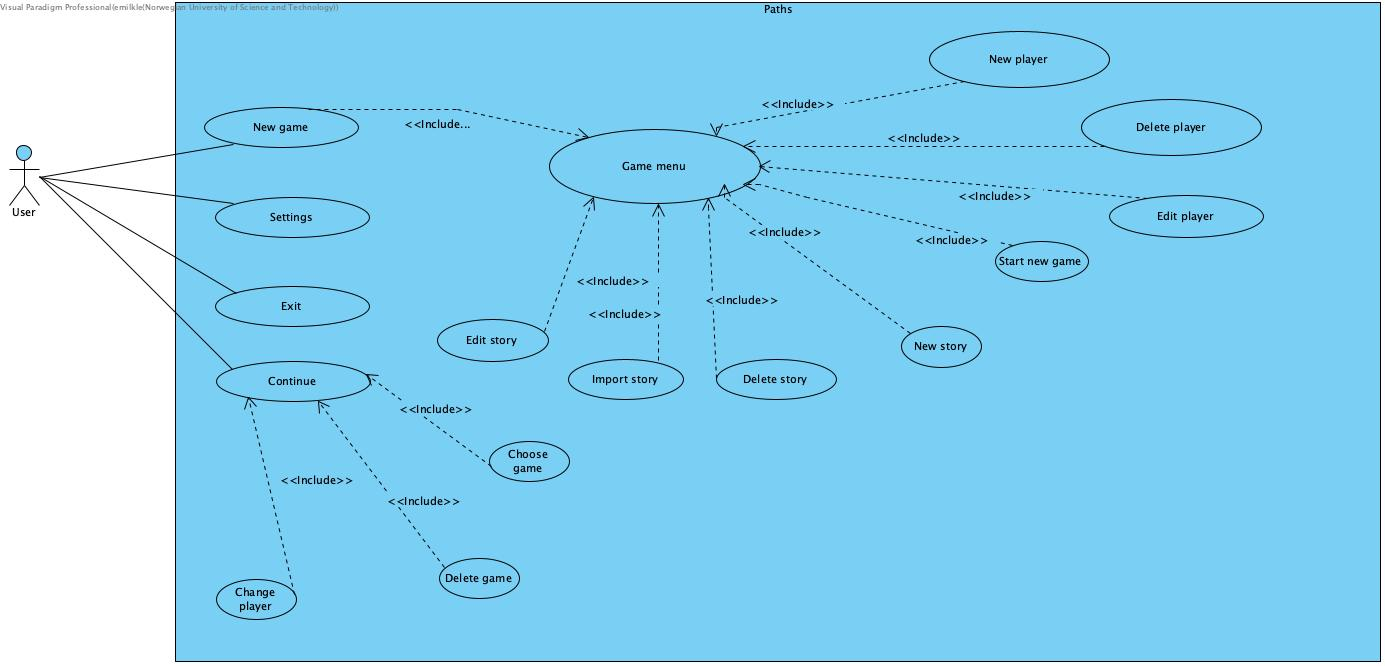
\includegraphics[width=1.3\textwidth]{figures/Paths_Use-Case.jpg} 
      }
    \caption
    {Paths use-case diagram. Source: Primary.}
\end{figure}
For the planning of the Paths game's requirements it became imminent to sketch our ideas by using a use-case diagram. In our diagram we included our plans for the overall layout of the application, with a start menu and also a new game menu. In the menu we planned to implement functionalities for choosing an already played game that you want to continue, a possibility to start a new game, a settings menu to change the language or audio in the game, and a functionality to exit the game. Then we planned, in some way or another, to have the possibility to start a new game from a ".paths" file, a way to delete a story and the player selected for the game, a way to create a new player and a new story as well as being able to have an overview of the game's dead links. The purpose of these functions is to make the game's layout similar to other narrative branching games, so the user can easily recognise the game in its functioning. 

\subsection{Technical Design}
%The technical design chapter describes the big picture of the chosen solution. For a software development project, this would typically contain the system arcitechture (client-server, cloud, databases, network- ing, services etc.); both how it was solved, and, more importantly, why this architecture was chosen.
To design this paths game, we have chosen to implement the functionality based on the MVC architectural pattern. The MVC helps the application's key components from interfering with each others tasks, and therefore creates an application with much more independent components. The implementation of this pattern was solved by firstly creating a package structure in our game, with one package for each component in the MVC. In the model package we chose to include classes like Story, Game, Passage, Link and the DAO classes that communicate with the database. For the rest of the application we created a ui package that contains the different views and their controllers in addition to the other GUI components like the dialog boxes and the story visualisers. For the paths Game the implementation of this pattern turns out to be very valuable, because it has been very easy to extend the application with new functionality, like for example the implementation of different languages. The languages got implemented easily by only changing the elements in the view that got shown at all times, like for example the text of buttons, the dialog boxes and the alerts got changed in the controller, so they could be activated in the correct case. 

\subsection{Development Process}
%In this chapter, you should describe the process that was followed. It should cover the process model, why it was chosen, and how it was implemented, including tools for project management, documentation etc. Depending on how you write the other chapters, there may be good reasons to place this chapters somewhere else in the report. 
Software development projects are rarely successful without using some sort of management tool to keep track of the development process. Therefore we have decided to use the GitLab issue board and the VCS system to help us keep track of who is doing what and to help us reach the goal in time. The issue board made it possible to create issues for each of the different functionalities we wanted to implement. The VCS system helped greatly in controlling the changes made to the program through the different commits made for each of the new code lines we added. We have also used documentation tools like Latex to write the main report of this project. Throughout the process we tried out pair programming, side by side, when implementing new functionality and when refactoring big parts of the program, so we both could get a greater understanding of the new additions to the code. These changes was often done on one PC at a time, so we could minimise the chance of merge conflicts.  
\\\\
Throughout the development process we have sometimes used generative AI models for different purposes. These models helped us save time by generating the main-menu background, saving us from the trouble of drawing it ourselves or finding a free-use picture. Another example of how we used these models is the pipeline on GitLab: we sadly did not have enough time to learn YAML from scratch, so we got a template from GitLab and had an AI model fine-tune it for our needs. Another use-case we had for AI models were troubleshooting database errors: as we have yet to learn about databases, the error logs were like hieroglyphs for us. The last area we used these models for were translating the resource bundles, as we only knew three of the five supported languages. It is important to state that we did not use generative AI models to develop the application, as we want to show our capabilities in the programming language we have learned for the past two semesters.

\newpage
\begin{figure}
\centering
\makebox[1 \textwidth][c]{ 
      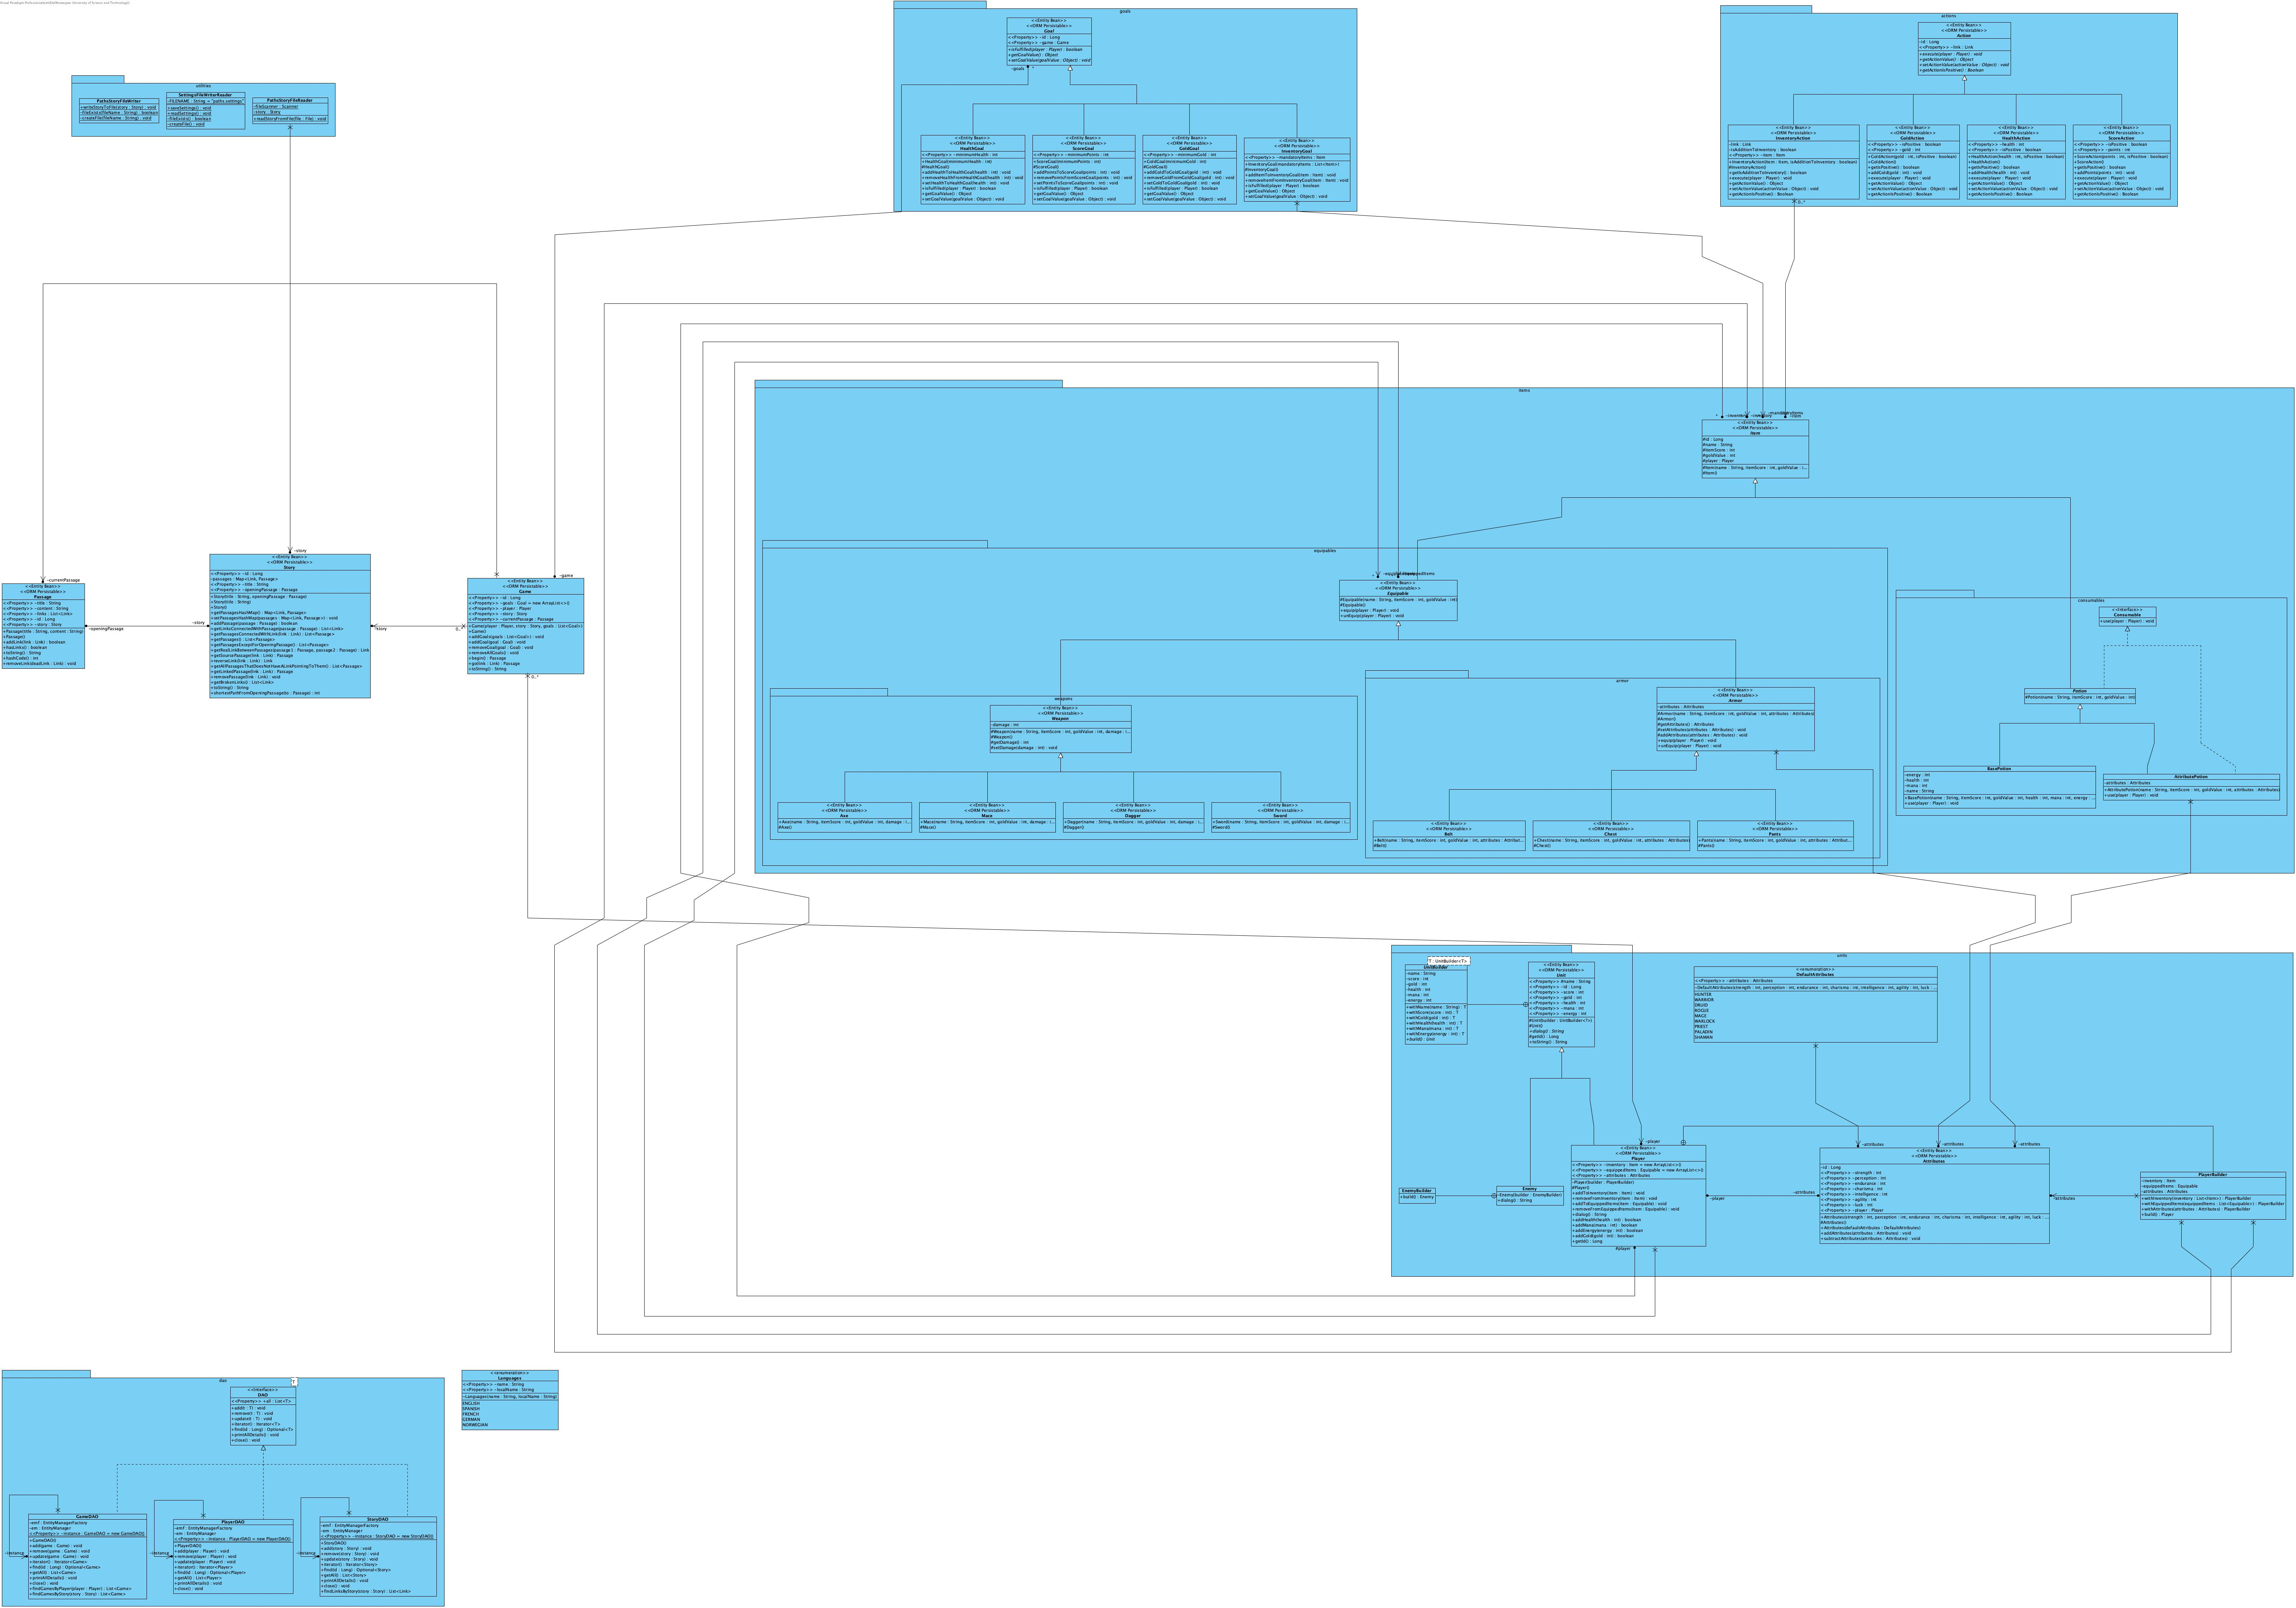
\includegraphics[width=1.3\textwidth]{figures/no.ntnu.idatg2001.paths.model.jpg} 
      }
    \caption
    {Paths model package class diagram. Source: Primary.}
\end{figure}

\begin{figure}
\centering
\makebox[1 \textwidth][c]{ 
      \includegraphics[width=1.3\textwidth]{figures/no.ntnu.idatg2001.paths.ui.jpg} 
      }
    \caption
    {Paths ui package class diagram. Source: Primary.}
\end{figure}

\newpage \pagebreak \cleardoublepage

\subsection{Implementation}
%Here you should describe the more technical details of the solution. Which tools were used (programming languages, libraries, IDEs, APIs, frameworks, etc.). It is a good idea to give some code examples. If class diagrams, database models etc. were not presented in the technical design chapter, they can be included here.
Paths got created using the Java programming language in the IntelliJ IDE, and also by implementing the Apache Derby Database. In addition we used the Junit framework for testing and CSS style sheets to be able to style the views exactly how we wanted. Above you can see two class diagrams of the Paths project drawn in Visual Paradigm. The first of the class diagrams shows the components situated in the model, the second diagram shows the components situated in the ui package, which consists of the programs controllers and the views. Within these packages we have created a inheritance hierarchy made of an interface called View that the views for the different parts of the game implement. 

%Give code examples here
\begin{figure}[H]
\centering
\makebox[1 \textwidth][c]{ 
      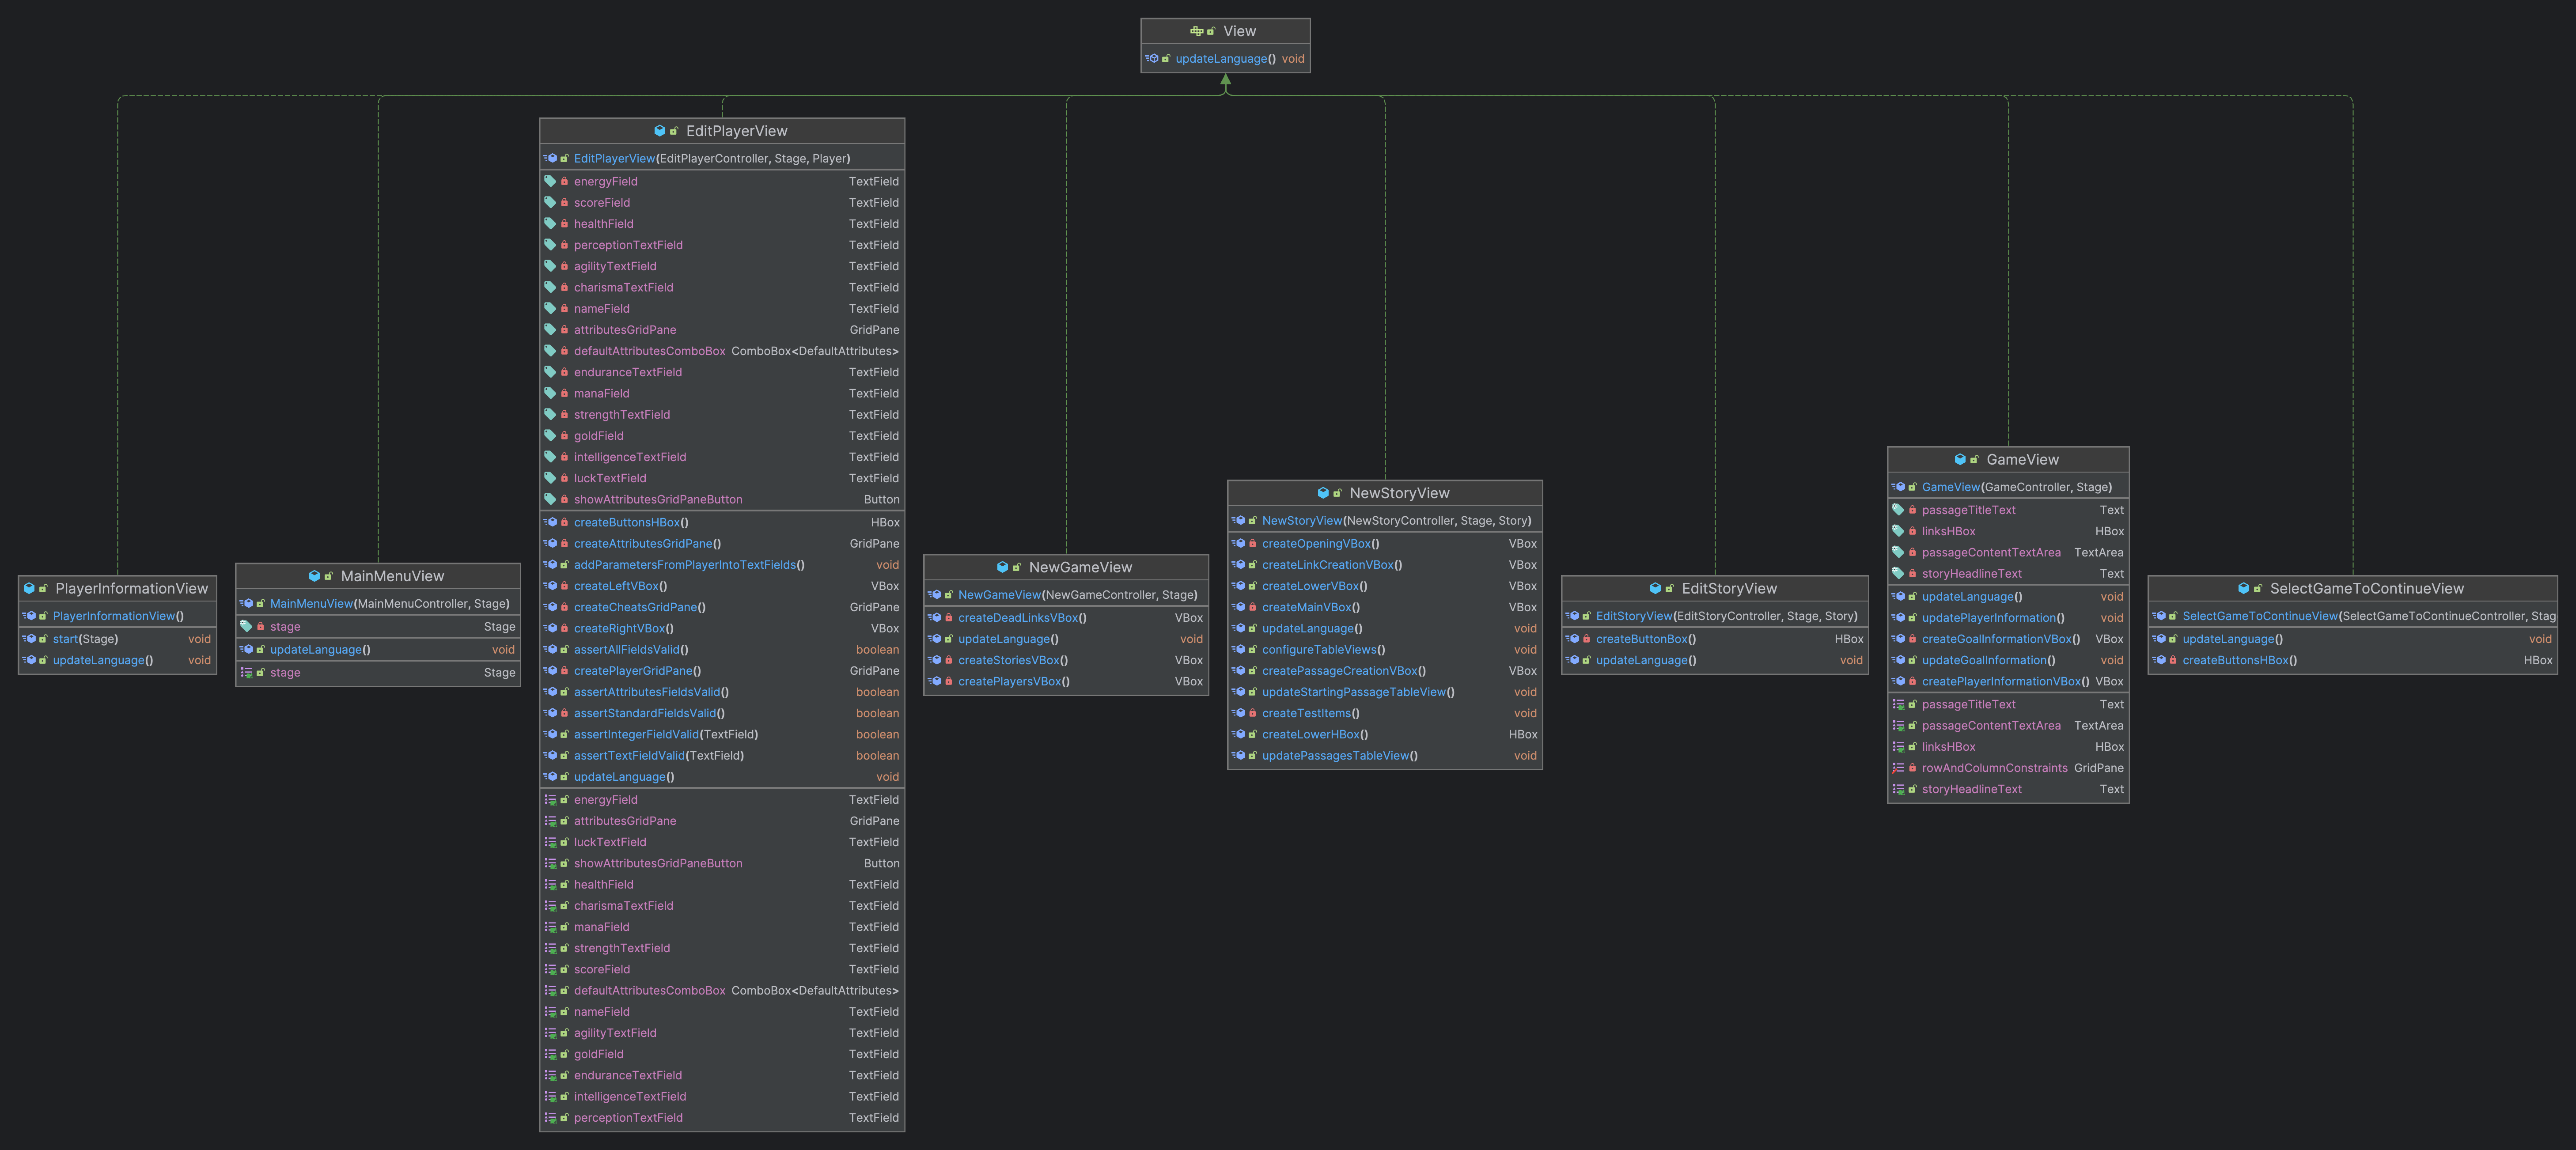
\includegraphics[width=1.3\textwidth]{views_package_v2.png} 
      }
    \caption
    {Paths view package diagram. Source: Primary.}
\end{figure}

\newpage

\begin{lstlisting}[language=Java,caption={View Interface. Source: Primary.}]
package no.ntnu.idatg2001.paths.ui.views;

import no.ntnu.idatg2001.paths.ui.controllers.Controller;

public interface View {
    void updateLanguage();
}
\end{lstlisting}

\begin{lstlisting}[language=Java,caption={MainMenuView class with View. Source: Primary.}]
package no.ntnu.idatg2001.paths.ui.views;

import java.io.IOException;
import java.util.Locale;
import java.util.Objects;
import java.util.ResourceBundle;
import javafx.application.Platform;
import javafx.geometry.Insets;
import javafx.geometry.NodeOrientation;
import javafx.geometry.Pos;
import javafx.scene.Scene;
import javafx.scene.control.Button;
import javafx.scene.image.Image;
import javafx.scene.layout.*;
import javafx.stage.Stage;
import no.ntnu.idatg2001.paths.model.dao.GameDAO;
import no.ntnu.idatg2001.paths.model.dao.PlayerDAO;
import no.ntnu.idatg2001.paths.model.dao.StoryDAO;
import no.ntnu.idatg2001.paths.ui.controllers.MainMenuController;
import no.ntnu.idatg2001.paths.ui.handlers.LanguageHandler;

public class MainMenuView implements View {
  private final MainMenuController controller;
  private final Stage stage;
  private final Button continueButton;
  private final Button newGameButton;
  private final Button settingsButton;
  private final Button exitButton;

  public MainMenuView(MainMenuController controller, Stage stage) throws IOException {
    this.controller = controller;
    this.stage = stage;

    stage.setTitle("Main menu");
    stage.setOnCloseRequest(
        event -> {
          event.consume();
          GameDAO.getInstance().close();
          StoryDAO.getInstance().close();
          PlayerDAO.getInstance().close();
          Platform.exit();
        });

    BorderPane root = new BorderPane();
    root.setPrefSize(1200, 800);

    AnchorPane centerPane = new AnchorPane();

    HBox centerHBox = new HBox();
    centerHBox.setAlignment(Pos.CENTER_LEFT);
    centerHBox.setNodeOrientation(NodeOrientation.RIGHT_TO_LEFT);

    HBox buttonsHBox = new HBox();
    buttonsHBox.setId("buttonsHBox");
    buttonsHBox.setAlignment(Pos.CENTER);
    buttonsHBox.setPrefSize(100, 200);
    buttonsHBox.setPadding(new Insets(5, 5, 5, 5));

    continueButton = new Button();
    newGameButton = new Button();
    settingsButton = new Button();
    exitButton = new Button();

    buttonsHBox.getChildren().addAll(continueButton, newGameButton, settingsButton, exitButton);

    AnchorPane.setBottomAnchor(centerHBox, 0.0);
    AnchorPane.setTopAnchor(centerHBox, 0.0);
    AnchorPane.setLeftAnchor(centerHBox, 0.0);
    AnchorPane.setRightAnchor(centerHBox, 0.0);
    centerPane.getChildren().add(centerHBox);

    root.setBottom(buttonsHBox);
    root.setCenter(centerPane);

    // CONTROLLER
    controller.configureContinueButton(continueButton);
    controller.configureNewGameButton(newGameButton);
    controller.configureSettingsButton(settingsButton);
    controller.configureExitButton(exitButton);

    // Observes when the language is changed, then calls updateLanguage()
    LanguageHandler.getObservableIntegerCounter().addListener((a, b, c) -> updateLanguage());
    updateLanguage();

    Scene scene = new Scene(root, 1200, 800);
    scene.getStylesheets().add("css/mainMenu.css");

    Image image =
        new Image(
            (Objects.requireNonNull(getClass().getResource("/images/PathsTitleScreen.png")))
                .openStream());
    BackgroundImage backgroundImage =
        new BackgroundImage(
            image,
            BackgroundRepeat.NO_REPEAT,
            BackgroundRepeat.NO_REPEAT,
            BackgroundPosition.CENTER,
            new BackgroundSize(1.0, 1.0, true, true, false, false));
    root.setBackground(new Background(backgroundImage));

    stage.setScene(scene);
    stage.show();
  }

  public Stage getStage() {
    return stage;
  }

  @Override
  public void updateLanguage() {
    ResourceBundle resources =
        ResourceBundle.getBundle(
            "languages/mainMenu",
            Locale.forLanguageTag(LanguageHandler.getCurrentLanguage().getLocalName()));

    // BUTTONS
    continueButton.setText(resources.getString("continueButton"));
    newGameButton.setText(resources.getString("newGameButton"));
    settingsButton.setText(resources.getString("settingsButton"));
    exitButton.setText(resources.getString("exitButton"));
  }
}
\end{lstlisting}
In this example you can see that each of the views are implemented with very specific characteristics and methods, except the updateLanguage method that they all override from the View interface. This makes it a much better design because the views will not contain loads of duplicated code lines. This is because each override of the updateLanguage method has its own signature with a specific resource bundle that all of the views GUI components will be translated by. 

\subsection{Deployment}
%This chapter should describe how your solution can be deployed on the employer’s system. It should include technical details on how to set it up, as well as discussions on choices made concerning scalability, maintenance, etc.
To run the Paths game on your own computer we have created a jar-file for the run configuration. This file can be run by opening it with the terminal command "java -jar 'path to file and name'.jar" on either a Mac, Windows or Linux operative system. 
\begin{lstlisting}[language=bash,caption={Mac version}]
    java -jar "filename".jar
\end{lstlisting}
\begin{lstlisting}[language=bash,caption={Windows version}]
    java -jar C: \Users\path-to-file.jar
\end{lstlisting}
\begin{lstlisting}[language=bash,caption={Linux version}]
    jar xf name-of-jar-file.jar [files-to-open]
\end{lstlisting}


\subsection{Testing}
%This chapter should describe how the system was tested during and after development. This would cover everything from unit testing to user testing; black-box vs. white-box; how it was done, what was learned from the testing, and what impact it had on the product and process.
When creating a software program you should not underestimate the power of testing and the many advantages it has. For the Paths project we have mostly focused on unit testing, since the project's scale is not suitable for more time-consuming and extensive testing like for example system testing and integration testing. Since our project is school project, we did not have any real product owner or stakeholders that were interested in the application that we could be employed by and communicate with. Therefore we did not take any consideration of user testing and user interviews. By unit testing we both learned much about the effect that testing could have on the development process when implementing new functionality. The effect really came to display when we tried to implement the file writer, since we could easily debug and test the code to see which part of the file writer that created an error. With the help of unit testing we also saved a lot of valuable time, since we were able to notice errors in early stages of the development process so we would not need to refactor everything nearing the end of the project. 

\subsection{Discussion}
%Here you should discuss all aspect of your report and project. How did the process work? Which choices did you make, and what did you learn from it? What were the pros and cons? What would you have done differently if you were to undertake the same project over again, both in terms of process and product? What are the societal consequences of your work?
To evaluate the project process it is important to both highlight the strengths and the shortcomings of the project. The main strengths of the project are related to the teamwork process and the overall flexibility of the game. This is because we believe we have together been able to learn fast from our mistakes and have good communication within the team. We have also been able to create a very flexible application thanks to the principles of the MVC and how it assisted the coupling and cohesion of the system. The shortcomings in the project mostly came from the problems with merge conflicts in the VCS system in GitLab at the start of the project, but as we became more comfortable with the VCS system we learned how to avoid it. If we were to undertake the same project over again we would most likely try to make our game available for more platforms so we could include as many users as possible and to satisfy a wider audience. 

\section{Conclusion}
%The conclusion chapter is usually quite short – a paragraph or two – mainly summarising what was achieved in the project. It should answer the claim part of the introduction. It should also say something about what comes next (‘future work’).
Throughout this project we have achieved many of the goals we had set at the start of the project. One of our main goals was to create a game based on other narrative branching game's mechanisms, but with a much simpler structure. We believe that we have achieved this in a good way by creating a GUI with a very simple layout and with stories that have endings based on your actions throughout the game. For later versions of this project, we have planned to implement some more time consuming functionality like 3D animations and support for more platforms, since that would require a lot of refactoring in the late stage of the project, which we would not have time to finish for this exam's due date. There is also some parts of the code that we would like to polish or develop further. One of these goals is a inventory system for items in the GUI, that would make for a better experience when playing the game. We would also polish the design of the GUI, since we valued functionality over looks. As we achieved many of the goals we had for our project, we are happy with the final product.

\bibliographystyle{ieeetr}
\bibliography{ref}

\LaTeX

\label{LastPage}
\end{document}